\section{Specifications}
\label{sec:specs}
\newcounter{SpecID}

\subsection{Markers}
\refstepcounter{SpecID}
\label{spec:markers}

The arena, and tokens, are labelled with fiducial markers. Each
marker number is associated with a particular feature in the arena,
and also has an associated size.  The marker numbers and sizes are
as follows:

\begin{center}
\begin{tabular}{lcc}
  \toprule
  \textbf{Item} & \textbf{Marker Number} & \textbf{Marker Size (\si{mm})} \\
  \midrule
  Arena boundary & 0 -- 27 & 250 \\
  Central reservation & 28 -- 39 & 250  \\
  % 28 to 31 reserved for robot badges
  Tokens & 100 -- 199 & 80 \\
  \bottomrule
\end{tabular}
\end{center}

\subsection{Arena}
\refstepcounter{SpecID}
\label{spec:arena}

\begin{enumerate}
  \item The arena floor is an \SI{8}{m} $\times$ \SI{8.1}{m} rectangle. The
        tolerance of these two dimensions is $\pm$ \SI{250}{mm}.
  \item The floor of the arena is carpeted.
  \item The layout of the arena is given in Figure~\ref{fig:arena}.
  \item The outer walls of the arena are at least \SI{600}{mm} high, and the
        interior surface is white plastic-coated hardboard.
  \item The outer track of the arena is \SI{1.5}{m} wide along the \SI{8}{m}
        edges, and \SI{1.55}{m} wide along the \SI{8.1}{m} edges.
  \item The central reserved area is surrounded by walls at least \SI{179}{mm}
        high.
  \item The starting location of the robots is given in Figure~\ref{fig:arena}.
        Teams are allowed to place their robot anywhere such that the entire
        robot is within \SI{1}{m} of the starting point, which will be
        indicated on the floor of the arena.
  % TODO: Spec the shortcut
  % TODO: Spec the supertoken pedestal
  \item The track boundaries are visually delineated on the floor of the arena
        by tape. The actual boundary is on the trailing edge of the tape --
        that is, a robot has passed the boundary when the back of the robot
        is past the tape.
\end{enumerate}

\begin{figure}
  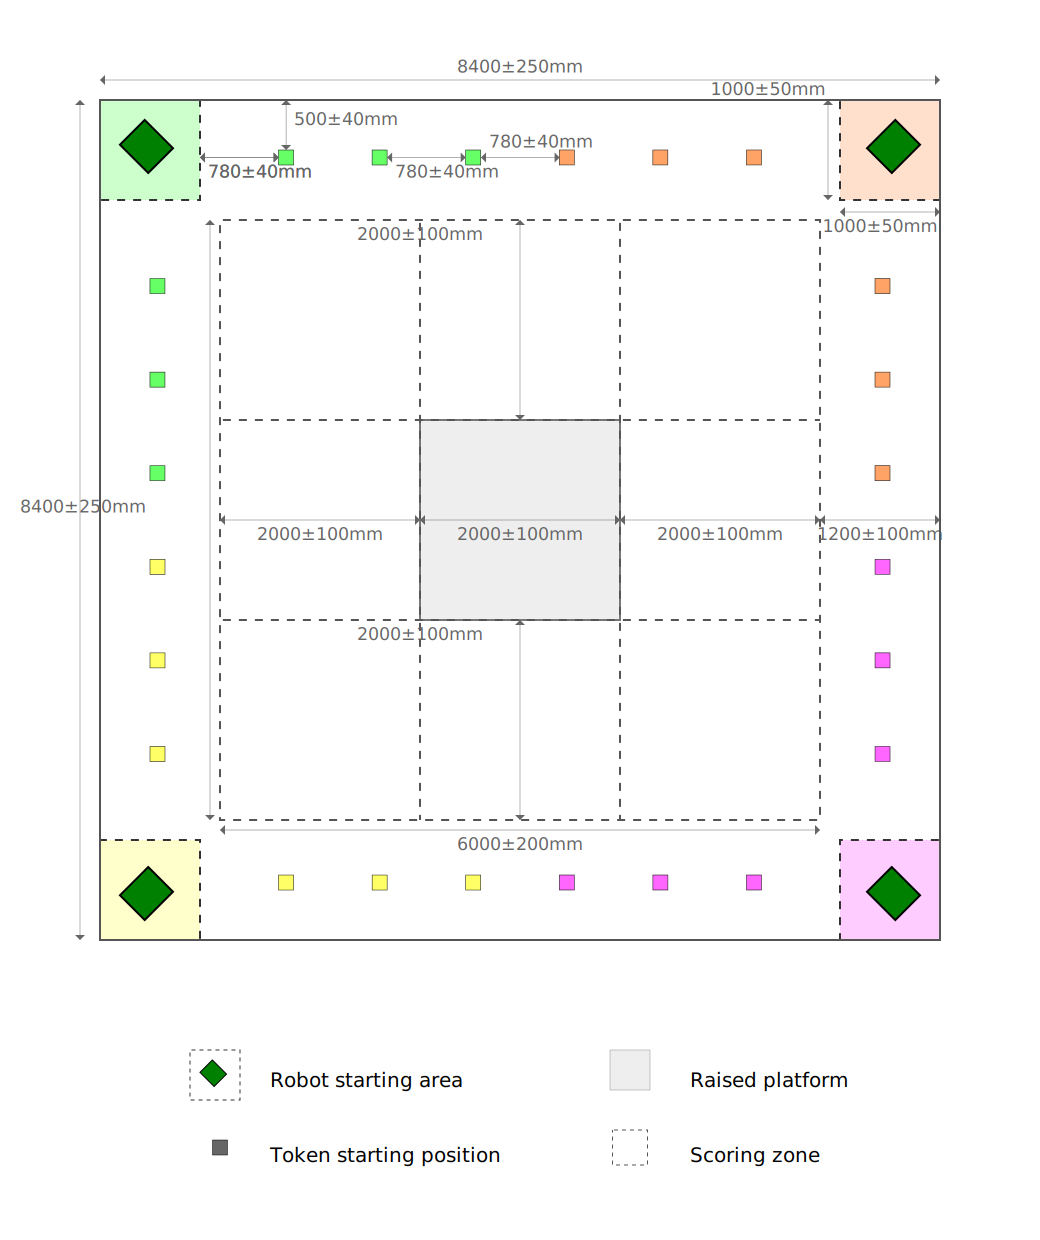
\includegraphics[scale=0.58]{fig-arena.pdf}
  \caption{Layout zones and cans in the arena.}
  \label{fig:arena}
\end{figure}

\subsection{Tin Cans}
\refstepcounter{SpecID}
\label{spec:cans}

\begin{enumerate}
  \item The tin cans are standard 400g steel tin cans, of height \SI{108}{mm}
        ($\pm$ \SI{5}{mm}), and radius \SI{75}{mm} ($\pm$ \SI{5}{mm}).
  \item The initial layout of tokens in the arena is given in
        Figure~\ref{fig:arena}.
  \item The tin cans are ferromagnetic.
\end{enumerate}

